%!TEX root = /Users/stevenmartell/Documents/CURRENT PROJECTS/iSCAM-trunk/docs/iSCAM-guide/overView.tex

\section{Running Examples} % (fold)
\label{sec:running_examples}
\begin{frame}
	\frametitle{Running examples}
	Examples in \texttt{iSCAM-trunk/examples}
	\begin{itemize}
		\item \texttt{Demo}
		\item \texttt{Hake}
	\end{itemize}
\end{frame}

\subsection{Demo Model} % (fold)
\label{sub:demo_model}


\begin{frame}
	\frametitle{Demo}
	\begin{itemize}
		\item The \texttt{Demo} directory is not present in the examples when you first checkout a copy of \iscam\ from the svn repository.
		\item To build the \texttt{Demo directory} cd to the examples directory and use \texttt{./makeproject Demo}
	\end{itemize}

\begin{figure}[htbp]
	\centering
		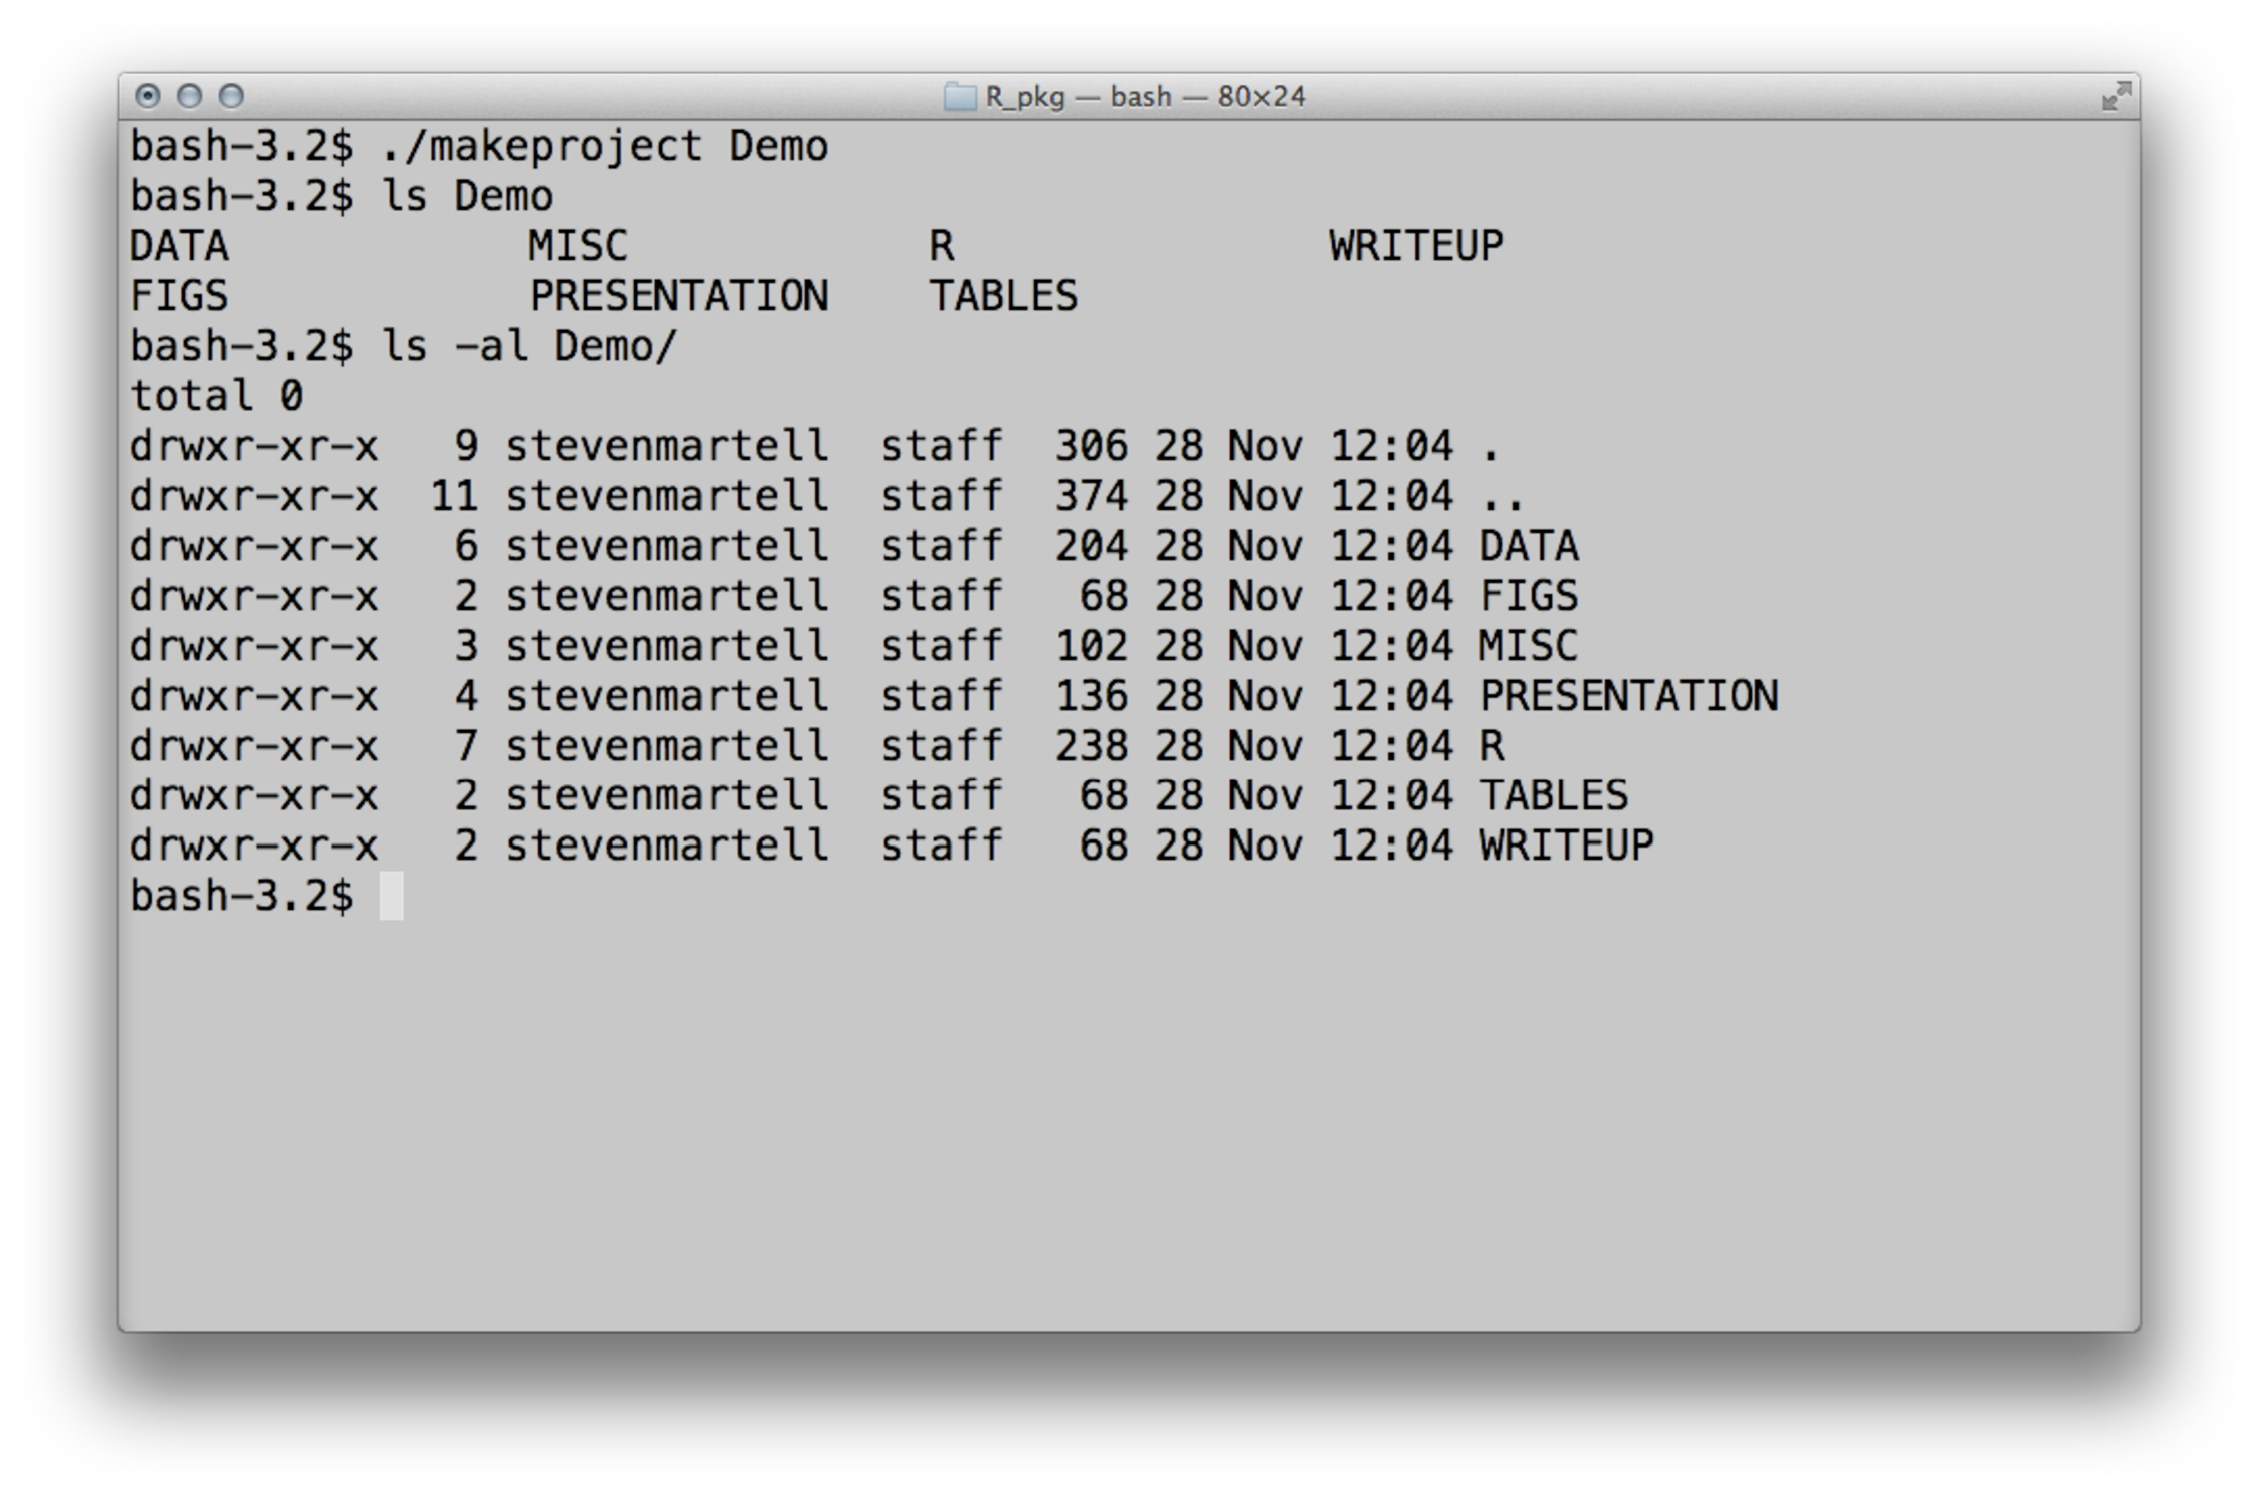
\includegraphics[height=1.75in]{screenCaptures/TermDemo.pdf}
	\caption{Using \texttt{makeproject} command to create \texttt{Demo}.}
	\label{fig:screenCaptures_TermDemo}
\end{figure}
\end{frame}

\begin{frame}
	\frametitle{Running the ADMB model in Demo}
	\begin{itemize}
		\item cd to the \texttt{examples/Demo/DATA} directory
		\item type \texttt{make} at the command line
	\end{itemize}
	\begin{figure}[htbp]
		\centering
			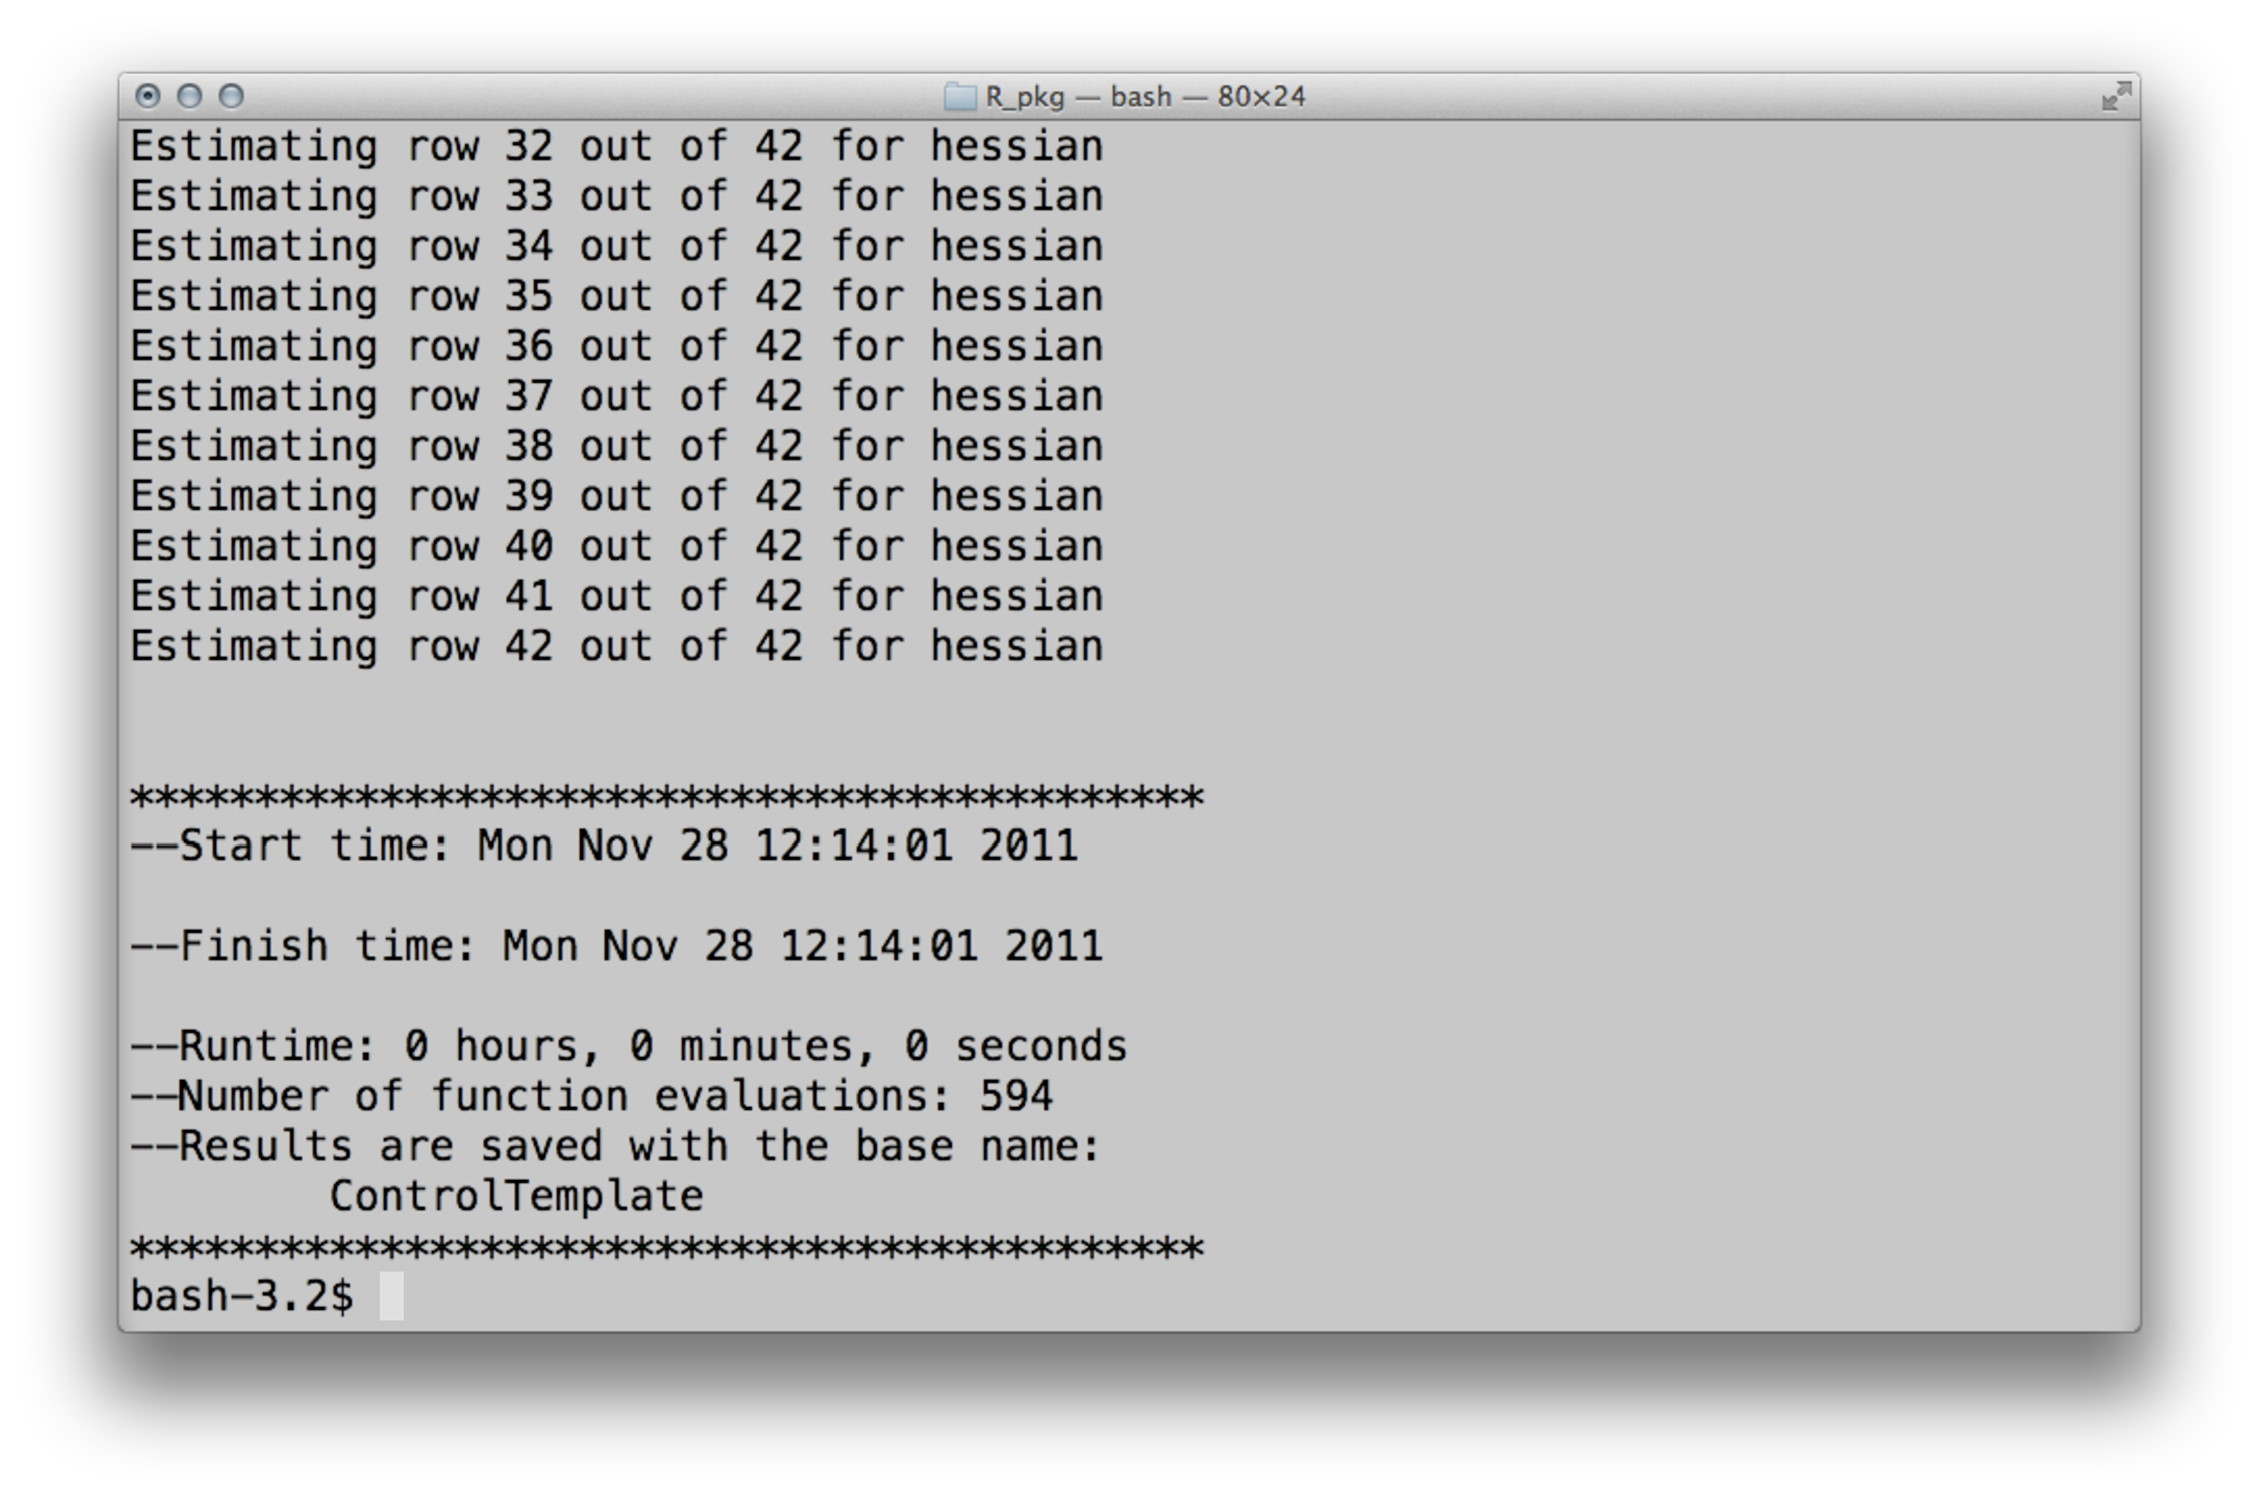
\includegraphics[height=1.75in]{screenCaptures/Term-catage.pdf}
		\caption{Terminal output after the Demo model has run}
		\label{fig:screenCaptures_Term-catage}
	\end{figure}
	
\end{frame}

% subsection demo_model (end)

\subsection{Makefile} % (fold)
\label{sub:makefile}
\begin{frame}[shrink=10]
	\frametitle{More on using \texttt{Makefile} }
	A makefile is a Unix utility that automatically executes a set of shell commands (rules). \underline{Target} rules are executed based on \underline{dependencies}.
	
	\begin{block}{Targets}
		\begin{itemize}
			\item all:  copy executable and run model with DAT \& ARG
			\item run:  copy executable and force a run
			\item mcmc: copy executable and run \texttt{mcmc} and \texttt{mceval}
			\item retro: copy executable and run retrospective R-script
			\item clean: remove executable \& other ADMB output files
		\end{itemize}
	\end{block}
	
	\begin{block}{Dependencies}
		\begin{itemize}
			\item EXEC - the name of the executable
			\item CTL - the name of the control file
		\end{itemize}
	\end{block}
	If the dependencies change then running make will execute the target scripts, otherwise there is no need to re-run the model.
\end{frame}

\lstset{language=make}
\begin{frame}[fragile]
	\frametitle{Setting up \texttt{Makefile}}
	User must supply variable Definitions in the Makefile:
	\begin{lstlisting}[cap=Makefile Defs]
	EXEC   = iscam
	prefix = ../../../dist
	DAT    = RUN.dat
	CTL    = ControlTemplate
	ARG    = 
	MCFLAG = -mcmc 10000 -mcsave 100 -nosdmcmc
	NR     = 4
	\end{lstlisting}
	\texttt{EXEC} is the program name, \texttt{prefix} is the (relative) path to the \texttt{dist} directory, \texttt{DAT} is the data file, \texttt{CTL} is the name of the control file, \texttt{ARG} optional command line argument (e.g., make run ARG="-nohess"), \texttt{MCFLAG} is the arguments for \texttt{make mcmc}, and \texttt{NR} is number of retrospective years (e.g., \texttt{make retro}). 
\end{frame}


\defverbatim[colored]\makesmart{%
\begin{lstlisting}[frame=single,emph={ga},emphstyle=\color{olive}]
bash-3.2$ make
make: Nothing to be done for `all'.
bash-3.2$  
\end{lstlisting}}%

\defverbatim[colored]\makearg{%
\begin{lstlisting}[frame=single,emph={ga},emphstyle=\color{olive}]
bash-3.2$ make run ARG = "-est -nox"
...
*******************************************
--Start time: Tue Nov 29 11:51:10 2011

--Finish time: Tue Nov 29 11:51:11 2011

--Runtime: 0 hours, 0 minutes, 1 seconds
--Number of function evaluations: 424
--Results are saved with the base name:
	ControlTemplate
*******************************************
bash-3.2$
\end{lstlisting}}%

\begin{frame}[fragile]
	\frametitle{Using \texttt{make} at the command line}
	\only<1>{
	Makefiles are smart, will only execute rules if the dependencies change:
	\vfill
	\makesmart
	}
	%%
	\only<2>{
	You can change the Makefile Defs at the command line:
	\vfill
	\makearg
	}
\end{frame}

\begin{frame}[fragile,shrink=30]
	\frametitle{Parallel execution with \texttt{Make}}
	Run multiple models in SUBDIR using: \texttt{make -j4}\\
	The "-j#" option specifies the number of processors to use.\\
	\texttt{SUBDIR} is the list of subdirectories in \texttt{DATA} (one for each model)\\
	\begin{lstlisting}[frame=single]
	## Makefile for running models
	## Author: steven martell <martell.steve@gmail.com>

	## Macros
	SUBDIR = CC PRD QCI SOG WCVI AREA27 AREA2W
	TARGET = 
	.PHONY: default $(SUBDIR) mcmc
	
	## Targets
	default: $(SUBDIR)
	$(SUBDIR):
		cd $@ && $(MAKE) $(TARGET)

	.PHONY: clean
	clean_files := $(foreach dir,$(SUBDIR),$(dir)/clean)

	clean: $(clean_files)
	$(clean_files):
		cd $(@D) && $(MAKE) clean
	\end{lstlisting}
	Sorry does not work on WINDOZE!
\end{frame}


% subsection makefile (end)

\begin{frame}
	\frametitle{Using \texttt{guiView}}
	In the R directory, source the iSCAM.R file in R $>$guiView()
	\begin{figure}[htbp]
		\centering
			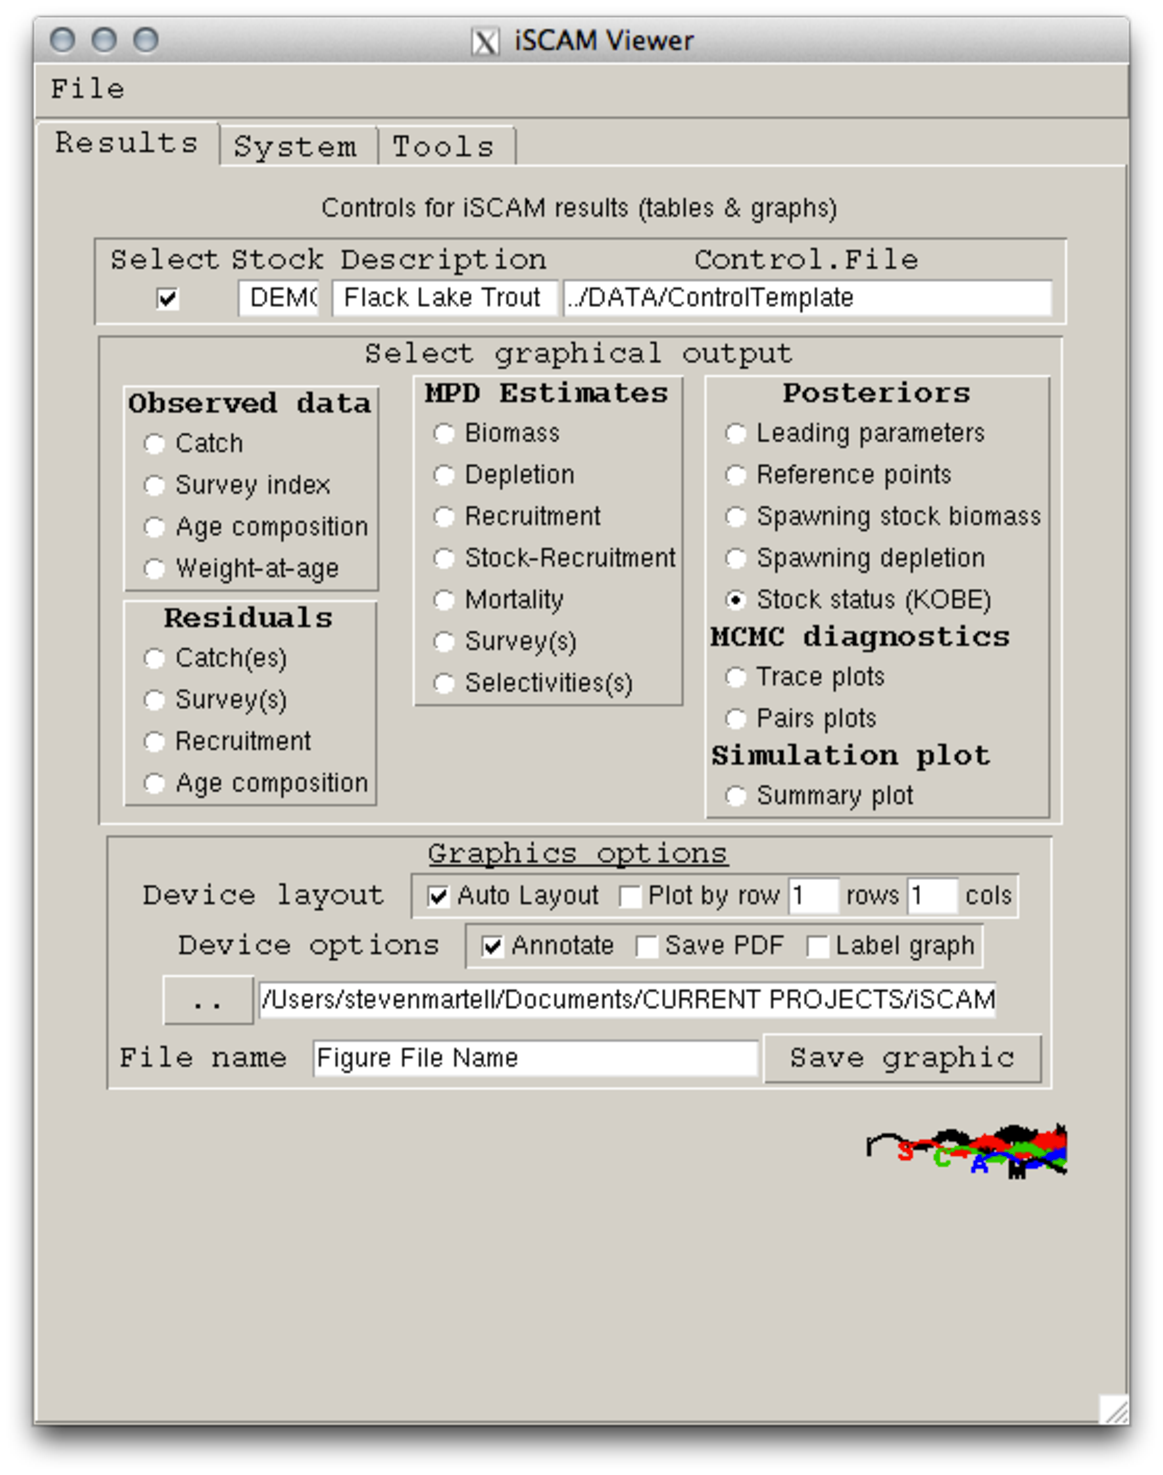
\includegraphics[height=2.5in]{screenCaptures/guiView.pdf}
		\caption{R gui for \iscam}
		\label{fig:screenCaptures_guiView}
	\end{figure}
	
\end{frame}


% section running_examples (end)